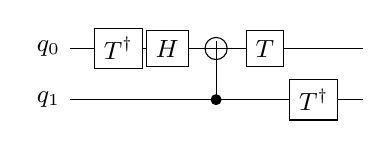
\begin{tikzpicture}[x=0.62cm,y=0.65cm, every node/.style={font=\small}]
\draw (0,0) node[left]{$q_0$} -- (6,0);
\draw (0,-1) node[left]{$q_1$} -- (6,-1);
\node[draw,fill=white,minimum size=0.43cm] at (1,0) {$ T^\dagger $};
\node[draw,fill=white,minimum size=0.43cm] at (2,0) {$ H $};
\draw (3,-1) -- (3,0);\fill (3,-1) circle (2pt);\draw (3,0) circle (4pt);\draw (3,0-.15)--(3,0+.15);
\node[draw,fill=white,minimum size=0.43cm] at (4,0) {$ T $};
\node[draw,fill=white,minimum size=0.43cm] at (5,-1) {$ T^\dagger $};
\end{tikzpicture}
